This section focuses on solving the underdetermined system derived in the previous section. To do this, SVD factorization will be used. \newline
We know that our system is composed of 36 equations for 59 unknowns. It is thus indeed underdetermined. Let us recap the strategy used to solve the system. We start with $$Ap=f.$$
We get the decomposition $$A = USV^{T}$$
with the properties from the course.
This yields
\begin{eqnarray*}
USV^{T}p & = & f\\
S\underbrace{V^{T }p}_{z} & = & \underbrace{U^{T}f}_{d}
\end{eqnarray*}
The matrix $S$ is diagonal and contains the singular values. We decide to keep the $r$ first (largest) singular values and set the other ones to zero. This correspond to looking for a least square solution in a subspace of $Col(A)$ but this reduces the sensitivity of the problem to data perturbations.


We set $z_{i}= d_{i}/s_{i}$ for $i = 1:r$. The other $z_{i}=0$ for $i = r+1,\dots,n$ give the minimum norm solution. Finally we recover the solution $p=Vz$ because we set $z=V^{T}p$ in the beginning.

\paragraph*{}
We look at the results we get without adding any noise to the data $f$. The codes are available at the end of the report. Here starts the game of finding the value of $r$ that works best. We must use enough information but not too much because the sensitivity of the system might cause problems. We first look at figure~\ref{fig:nn0} where we tried the values $r= \begin{bmatrix}
1 & 10 & 20 & 30 
\end{bmatrix}$
We see that $r=1$ does not suffer any oscillation but clearly does not use enough informations. The value $r=10$ gives an acceptable result. Oscillations start to appear at $r=20$ and there are many more at $r=30$.
\begin{figure}[!h]
\centering
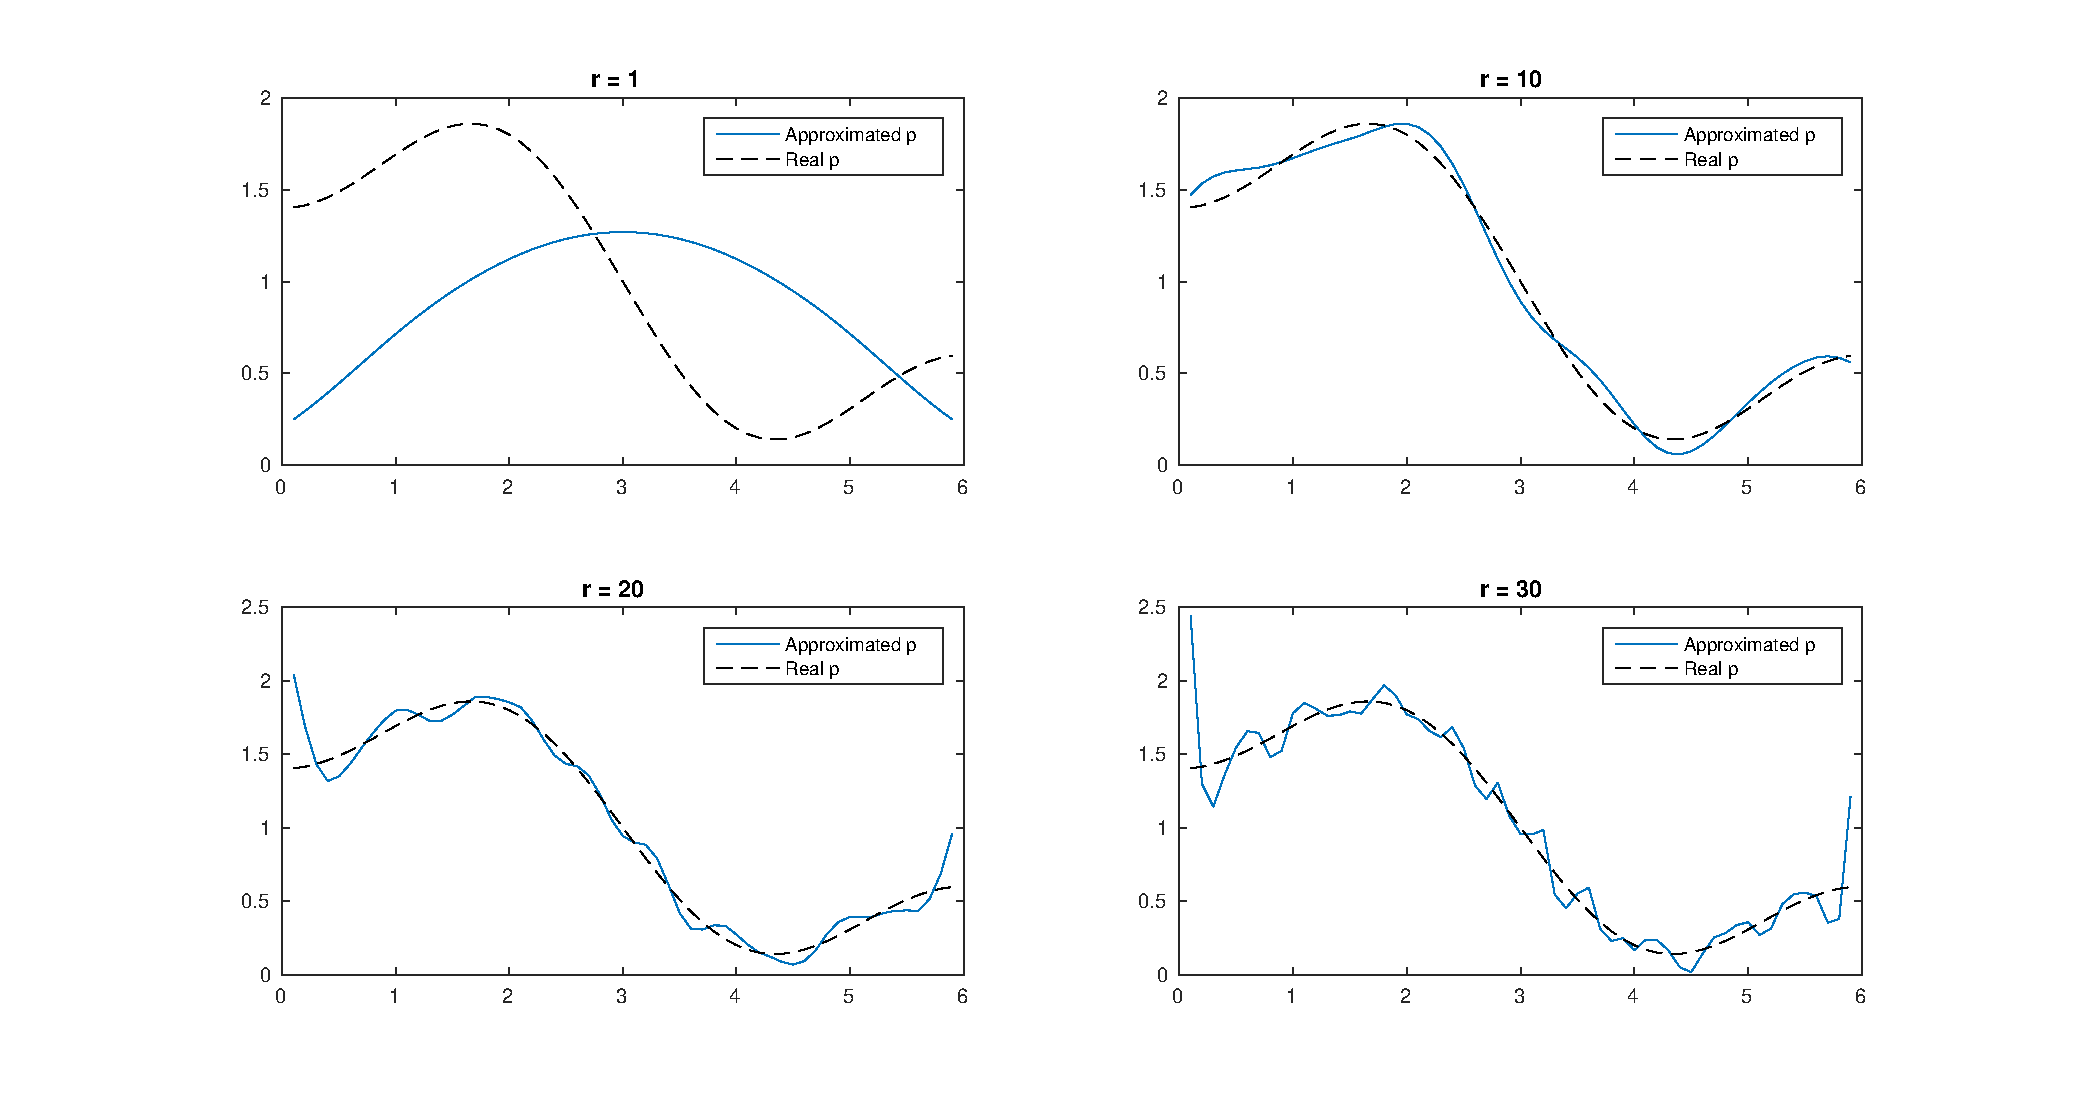
\includegraphics[scale = 0.5]{./nn0.eps}
\caption{Results for some values of $r$}
\label{fig:nn0}
\end{figure}

Printing the results for other values of $r$, we see that the best fitting curve is obtained around $r=10$. On figure~\ref{fig:nn2} we have the best results possible. To choose a value for $r$, one might have to fix a criteria. It could be, for example, the square error or the maximum difference between the two curves. We won't go into this kind of details but it seems that $r=9$ or $r=10$ both give equally great approximation.

%\begin{figure}[!h]
%\centering
%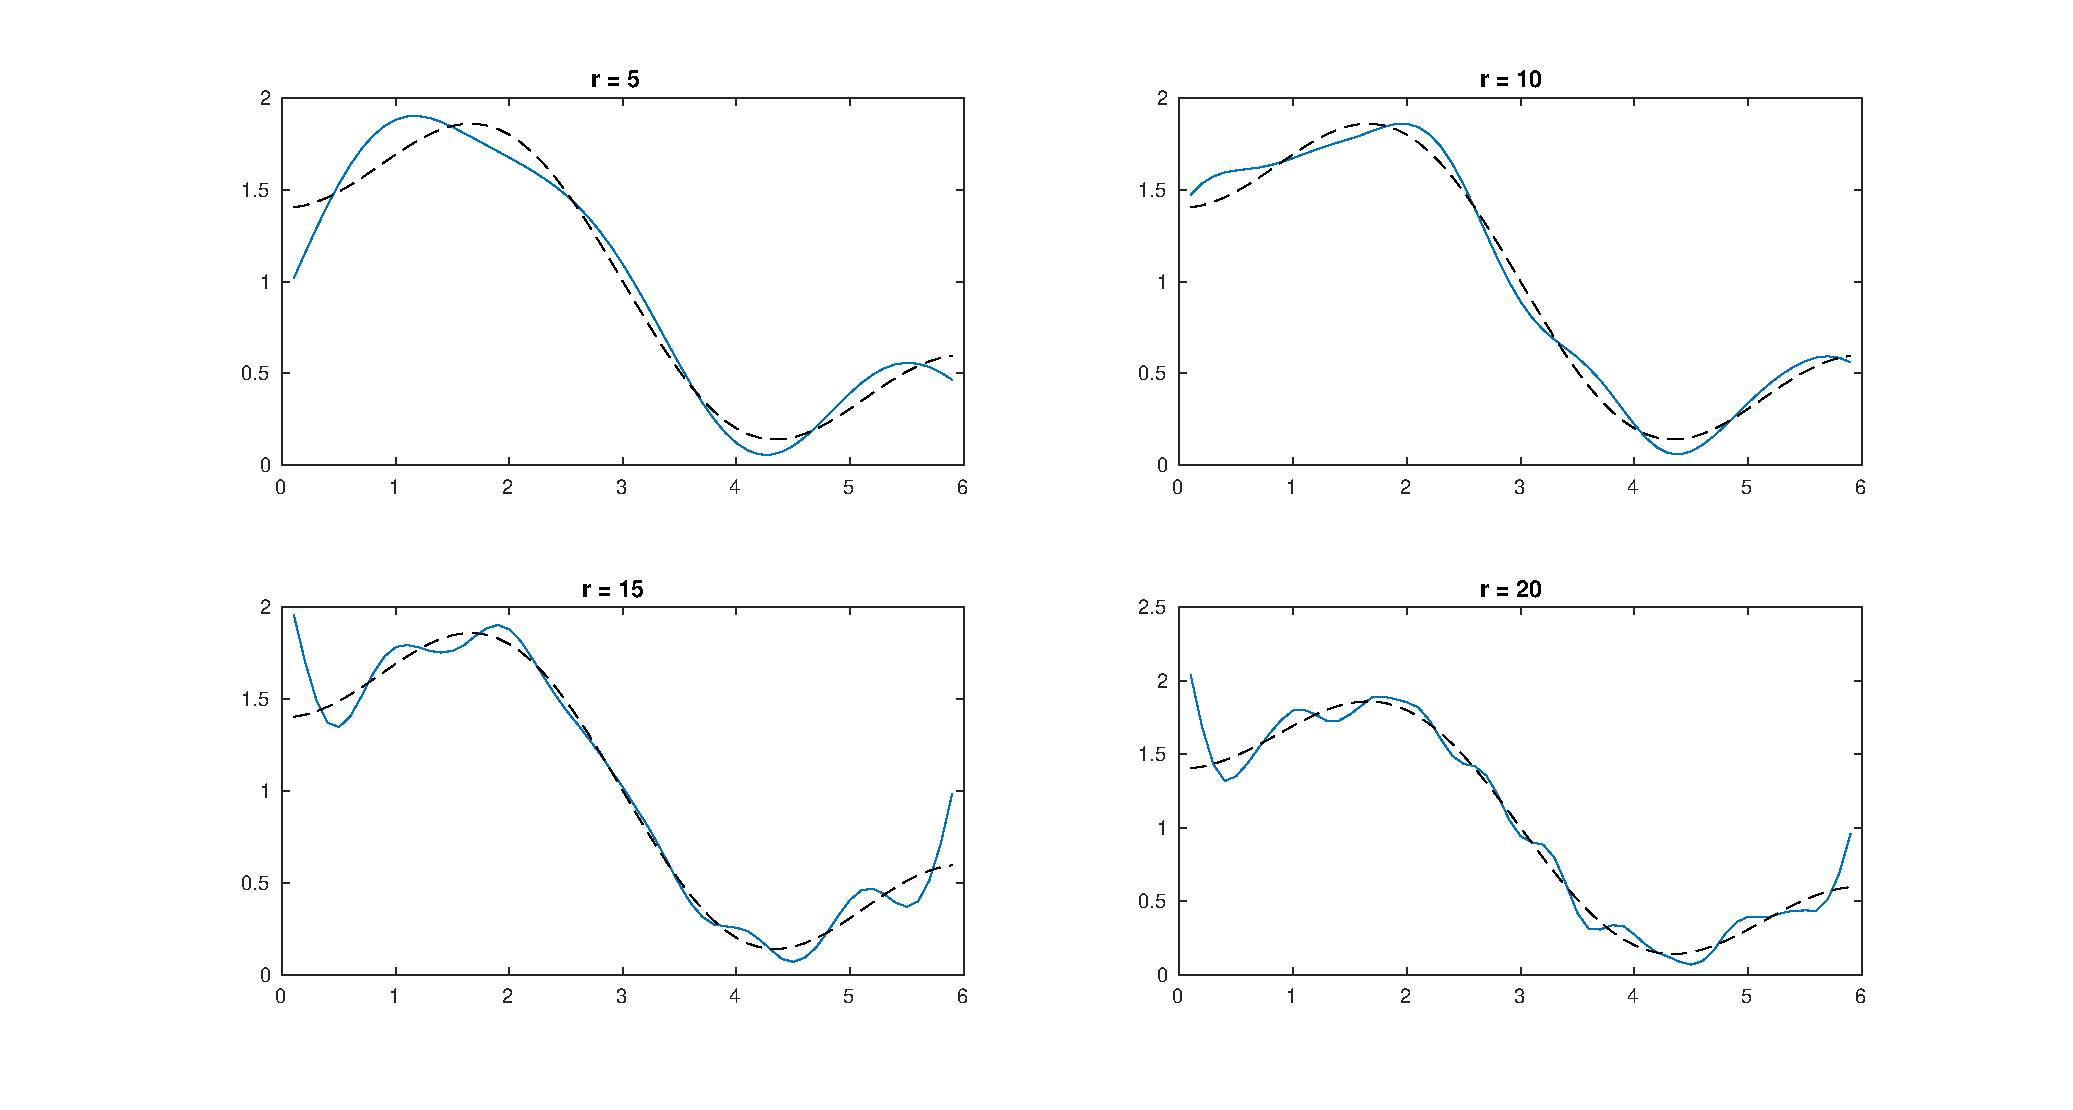
\includegraphics[scale = 0.5]{./nn1.eps}
%\caption{Results for some values of $r$}
%\label{fig:nn1}
%\end{figure}

\begin{figure}[!h]
\centering
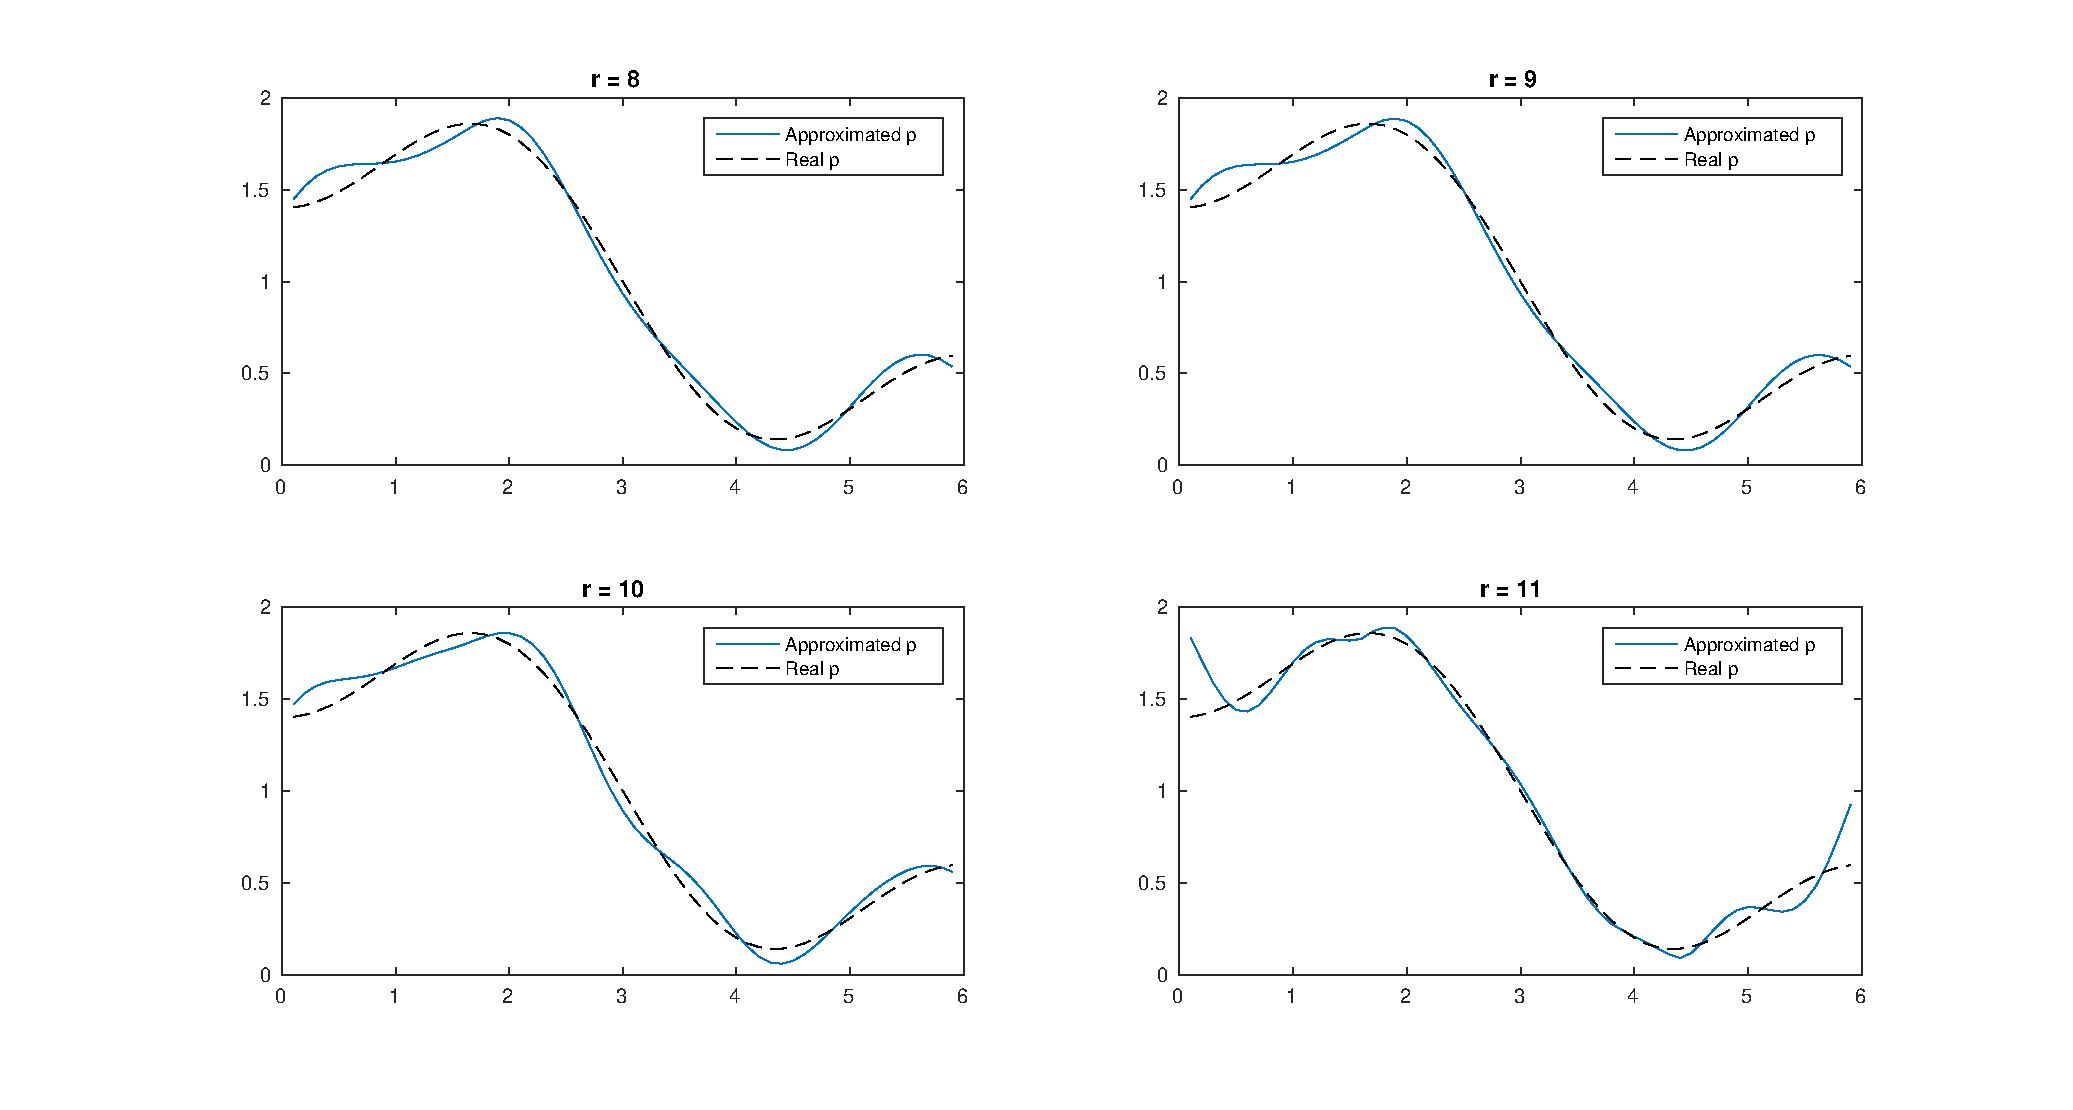
\includegraphics[scale = 0.5]{./nn2.eps}
\caption{Results for some values of $r$}
\label{fig:nn2}
\end{figure}



